\documentclass[12pt]{article}

\usepackage{amsmath}    % need for subequations
\usepackage{graphicx}   % need for figures
\usepackage{verbatim}   % useful for program listings
\usepackage{color}      % use if color is used in text
\usepackage{subfigure}  % use for side-by-side figures
\usepackage{hyperref}   % use for hypertext links, including those to external documents and URLs

\author{P.~Gusev}
\title{NdnRTC app design and protocol specification (DRAFT v0.1)}

\begin{document}

\maketitle
\newpage

%************************************************
\section*{Abstract}
\tableofcontents

\newpage
\section{Overview}
\subsection{Participants and institutions}
\begin{itemize}
\item Jeff Burke
\item Jeff Thompson
\item Peter Gusev
\item Qiuhan Ding
\end{itemize}

\subsection{Description}
Video conferencing tool is one of those apps, which is needed first of all for internal use and experimenting with real-time communication over NDN. As we are interested in increasing NDN popularity among non-research peers as well, we are trying to provide easy-to-setup NDN-apps by employing web-browser APIs. NDN-WebRTC is a JavaScript application which utilizes WebRTC engine for media encoding/decoding and C++ NDN library for transport layer. Proposed initial app design contained two main modules: 
\begin{enumerate}
\item \textbf{Browser add-on} \\
Contains NDN media-specific transport layer implementation, encoding/decoding engine (WebRTC) and provides JavaScript API for the access from the browser apps;
\item \textbf{JavaScript app} \\
Provides general conference discovery between peers
\end{enumerate}

The app borrows some ideas from previous works \cite{videoTR,ChronosTR}. It maintains synchronization of digest tree in order to keep track of current chat participants in the same manner as ChronosChat \cite{ChronosTR}. Given that information, new participant can start fetching media data objects from other peers (according to media namespace presented on Figure \ref{media-ns}).

\begin{figure}
\centering
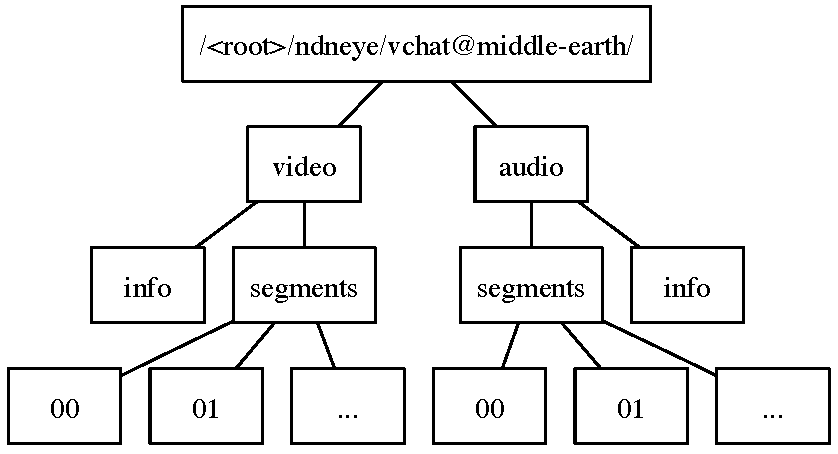
\includegraphics[width=0.8\textwidth]{../res/graphics/namespace-v01}
\caption{NDN-WebRTC Media Namespace}
\label{media-ns}
\end{figure}

The main goal of fetching media is to minimize the delay of receiving latest frames. Having that in mind, we came up with the following design assumptions:

\begin{itemize}
\item Consumers are in full control of the speed of issuing media interests (i.e. interests in a segments namespace);
\item Most recent media frames are delivered by pipelining media interests at a priori higher rate than producer delivers them (since the peer can obtain framerate information from the other peer by questioning "info" namespace, it can determine frequency of interest issuing);
\item The presence of outstanding interests indicates retrieval of the most recent data;
\item If consumer has no outstanding interests, it increases interest rate or, depending on the average rendering time, switches to a lower media quality. 
\end{itemize} 

Since no synchronization problems need to be solved in such "consumer" approach, we hope that NDN-WebRTC can show better results in scalability for many-to-many scenarios.

\subsection{Next steps}
\begin{itemize}
\item Provide user authentication in video conferences
\item Implement secure media transfer
\item Scalable video encoding
\end{itemize}

\section{Protocol specification}
\subsection{Intro}

\subsection{Discovery}
\textit{TBD}

\subsection{Negotiating}
\begin{enumerate}
\item Upon successful discovery of a video producer URI Consumer issues interest in index namespace and gets data about media streams parameters ($FrameRate$ and codecs).
\item Consumer issues $Index_{0}$ with \textit{RigthMostChild=\textbf{true}} selector in frames namespace like this: \textit{/root/mediadata} and waits unless first segment is not received.
\item Consumer switches to \textbf{"Chase Mode"}
\end{enumerate}

\textbf{Chase Mode}
\begin{enumerate}
\item Consumer extracts frame number - $FN$ from the obtained $DataObject$ and pipelines interests for  at $2*FrameRate$ rate (twice faster than consumer data rate) with \textit{RightMostChild=\textbf{true}} in segments namespace like this: \textit{/root/mediadata/FN/0}. i.e. pipeline contains interests $Index_{FN}$, $Index_{FN+1}$, $Index_{FN+2}$,...

\item Consumer watches two parameters: $DeliverRate$ of frames, $RoundTripTime$ for interests:
\begin{itemize}
\item If $DeliverRate$ is the same as $FrameRate$  and $RoundTripTime$ is not growing steadily, Consumer switches to \textbf{Fetch Mode} (see below)
\item If either $DeliverRate$ and/or $FrameRate$ are growing, Consumer chooses lower quality (by modifying prefix) and re-enables \textbf{Chase Mode}
\end{itemize}
\end{enumerate}

\textbf{Fetch Mode}
\begin{enumerate}
\item Consumer extracts the latest frame number - $LFN$ and sets up a \textit{Frame interest} pipeline at $2*FrameRate$ frequency:
\begin{center}
for a 24 fps video:
\begin{itemize}
\item \textbf{t = 0 sec} \\
Interest for \textit{/root/video/LFN/0}, timeout = 1.5 sec
\item \textbf{t = 1/48s} \\
Interest for \textit{/root/video/LFN+1/0}, timeout = 1.5 sec
\item \textbf{t = 2/48s} \\
Interest for \textit{/root/video/LFN+2/0}, timeout = 1.5 sec
\item ...
\end{itemize}
\end{center}

The number of segments per frame ($SegNum$) is indicated using \textit{FinalBlockID} field of each segments' DataObject. Consumer sets up \textit{Segments interest} pipeline for each frame interest like this: 
\begin{center}
\begin{itemize}
\item Interest for \textit{/root/video/LFN/0}
\item Interest for \textit{/root/video/LFN/1}
\item Interest for \textit{/root/video/LFN/2}
\item ...
\item Interest for \textit{/root/video/LFN/$SegNum$}
\end{itemize}
\end{center}

\item Consumer periodically issues \textbf{"probe"} interest with the last known frame number and \textit{RightMostChild=\textbf{true}} in order to detect lag from producer. If considerable lag was detected, Consumer chooses lower stream parameters and switches to the \textbf{Chase Mode}

\item Consumer watches the value of $DeliveryRate$ and $RoundTripTime$ for the interests. If either of these values start to grow, Consumer should choose lower stream parameters and switch  to the \textbf{Chase Mode} in order to minimize lag from producer.

\end{enumerate}

\section{App design}
Figure \ref{fig:uc} represents common use cases for the add-on. Currently, use case \textit{Discover conferences} is left for future development.
\begin{figure}
\centering
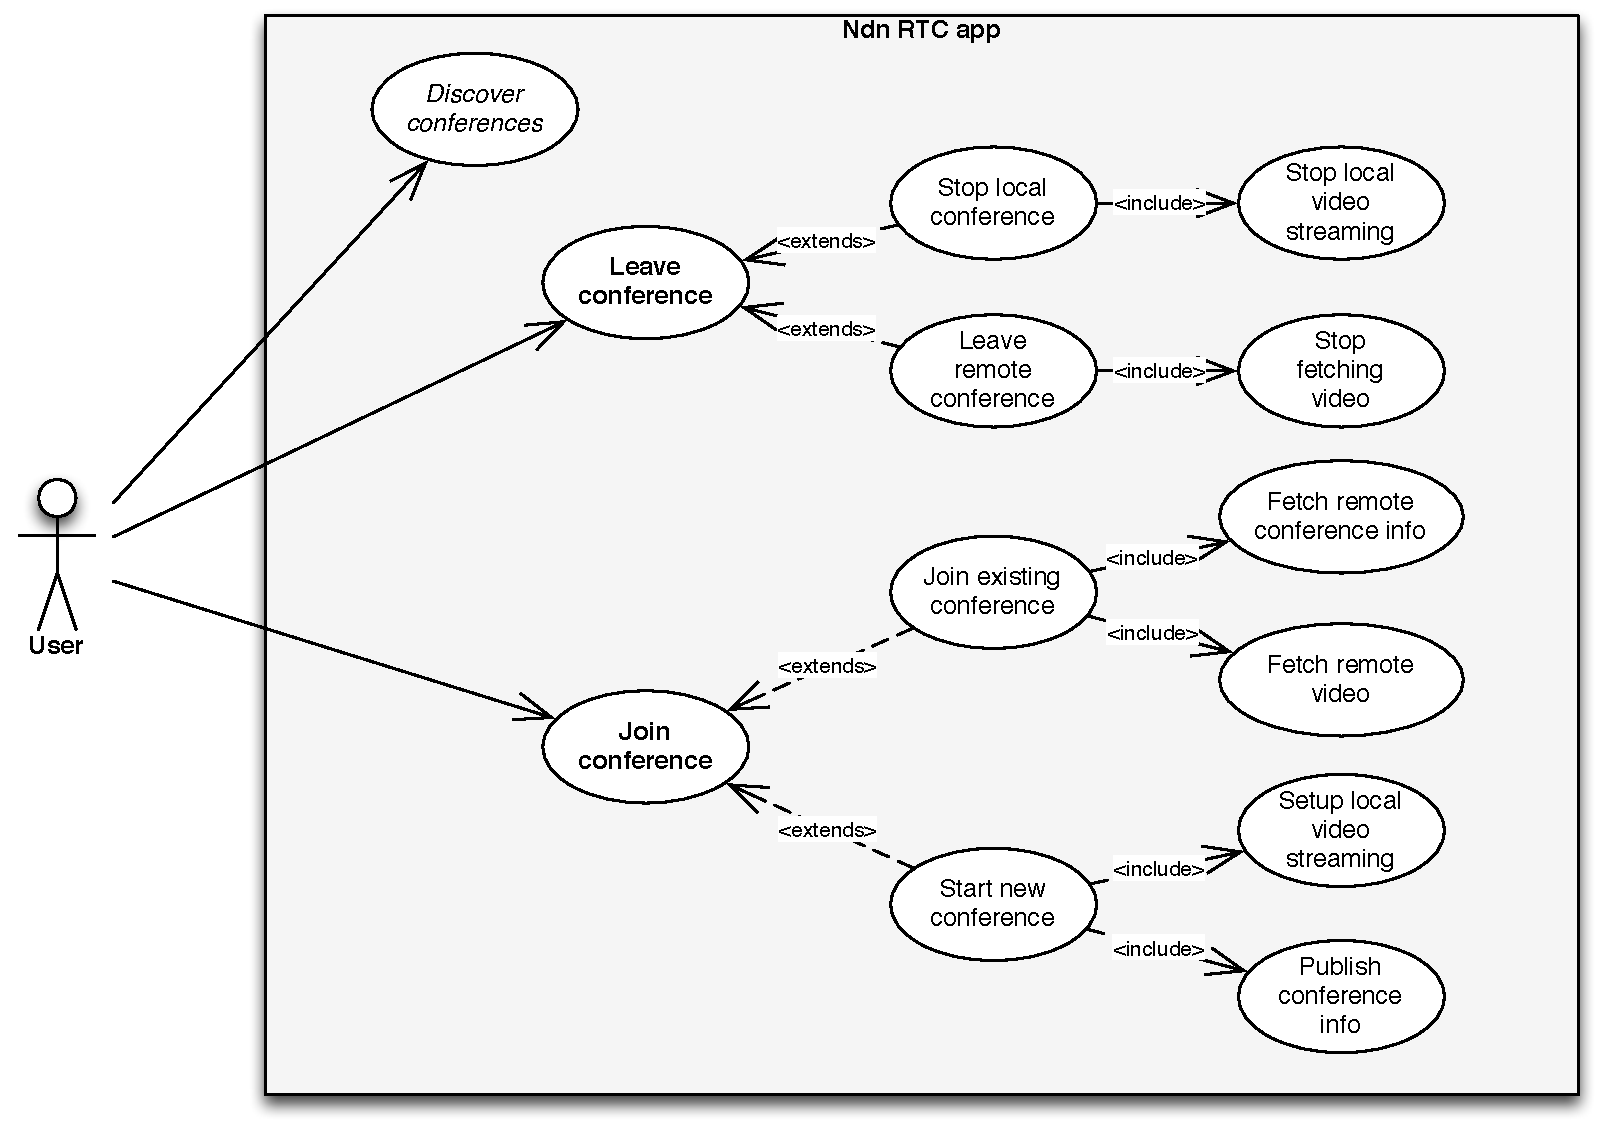
\includegraphics[width=\textwidth]{../res/graphics/addon-uc}
\caption{Add-on Use-Cases}
\label{fig:uc}
\end{figure}


Top-view architecture of add-on is presented on Figure \ref{fig:arch}.
\begin{figure}
\centering
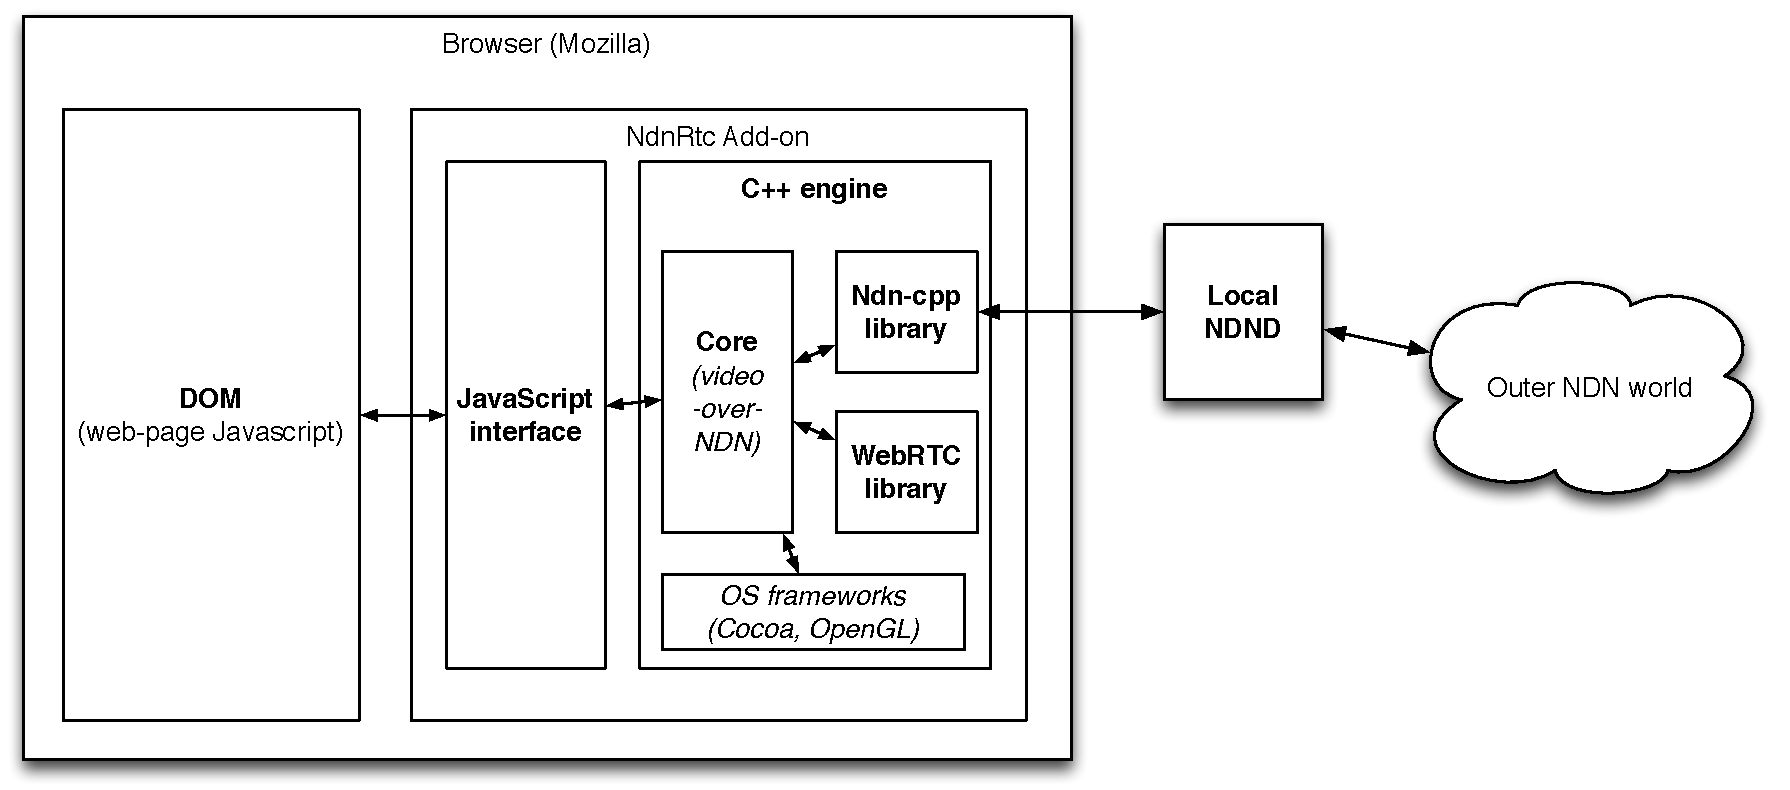
\includegraphics[width=\textwidth]{../res/graphics/addon-arch}
\caption{Add-on architecture}
\label{fig:arch}
\end{figure}

\subsection{C++ XPCOM add-on}
This sections describes internal architectural approach for C++ part of add-on.

One can start learning how add-on works by looking of sequence diagrams of main use-cases: Starting a conference (Figure \ref{fig:start}), Joining existing conference (Figure \ref{fig:join}) and Leaving a conference (Figure \ref{fig:leave}).

\begin{figure}
\centering
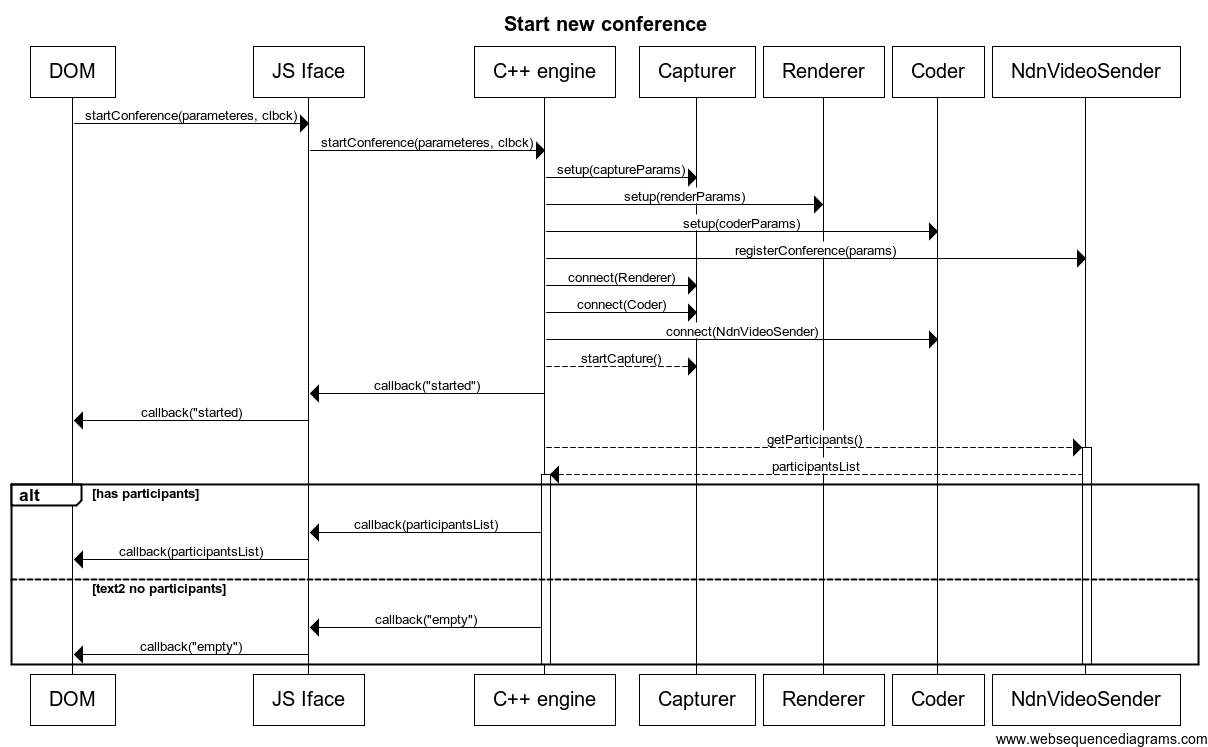
\includegraphics[width=\textwidth]{../res/graphics/start-seq}
\caption{Sequence diagram for starting a conference}
\label{fig:start}
\end{figure}

\begin{figure}
\centering
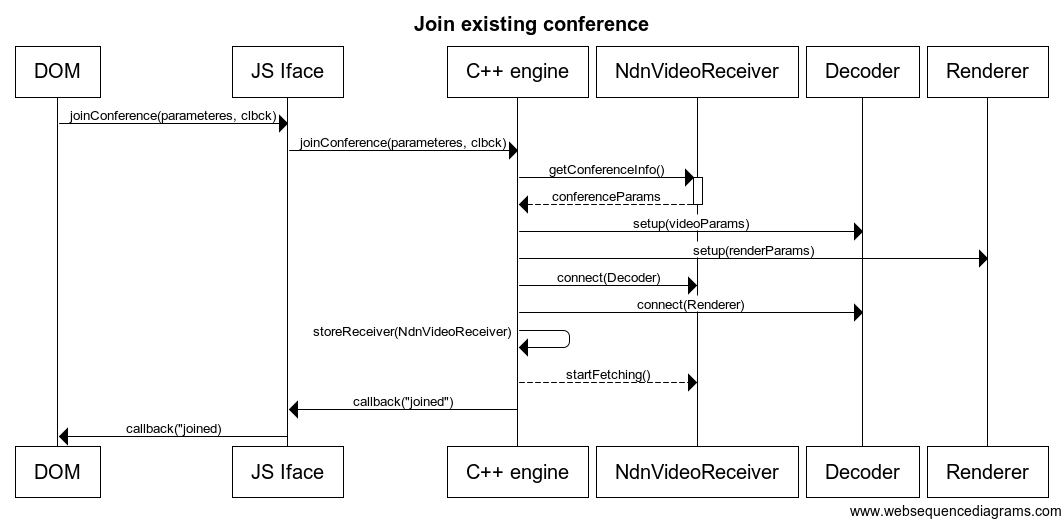
\includegraphics[width=\textwidth]{../res/graphics/join-seq}
\caption{Sequence diagram for joining existing conference}
\label{fig:join}
\end{figure}

\begin{figure}
\centering
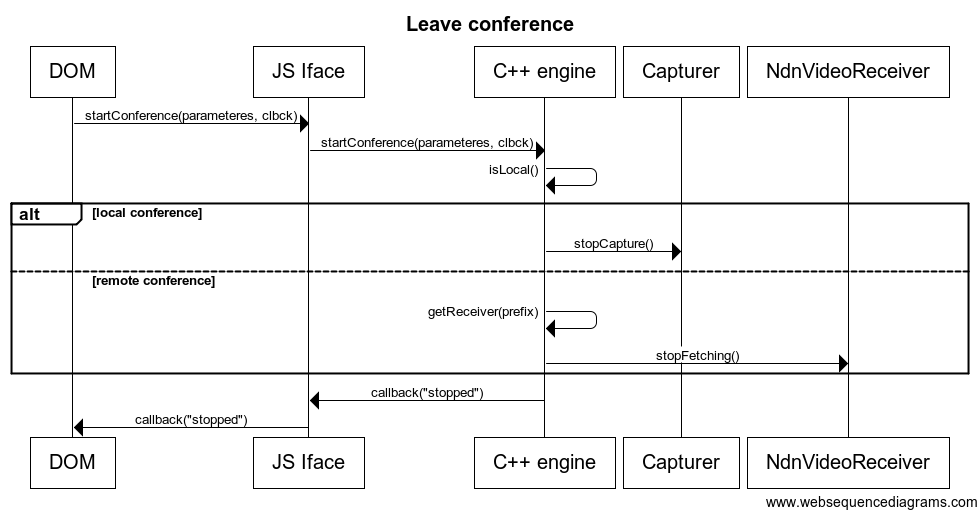
\includegraphics[width=\textwidth]{../res/graphics/leave-seq}
\caption{Sequence diagram for leaving a conference}
\label{fig:leave}
\end{figure}


\subsection{Javascript Web application}

\section{References} \cite{videoTR}, \cite{ChronosTR}
%************************************************
\bibliography{../res/bib/ndn-np}
\bibliographystyle{plain}



\end{document}